\section{Benchmark}

\subsection{Max-cut}

% \begin{figure}[H]
% \centering
% 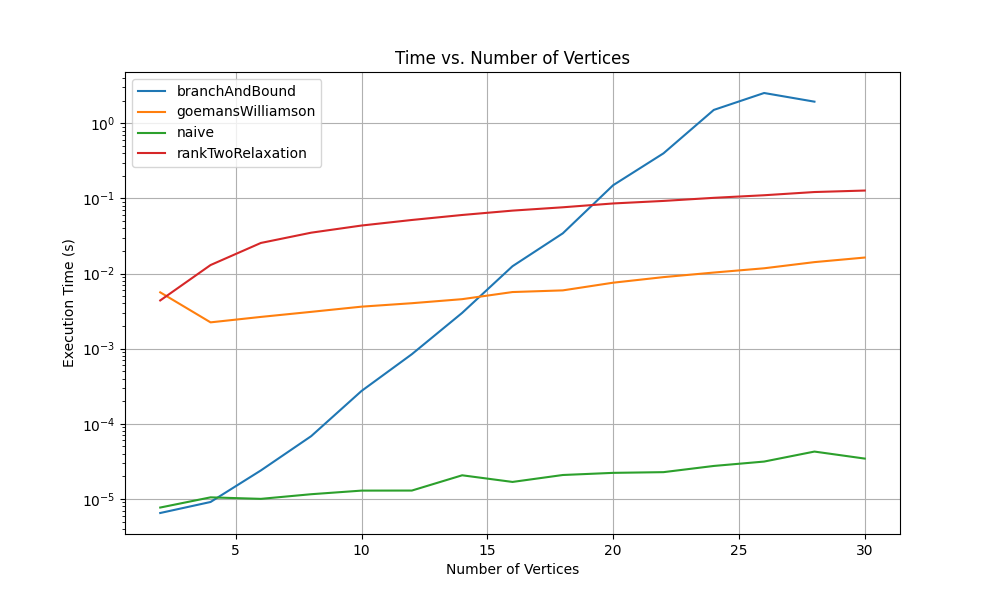
\includegraphics[width=\textwidth]{chapters/benchmark/Sections/images/cut/small_graphs/time_vs_vertices.png}
% \end{figure}

\begin{figure}[H]
\centering
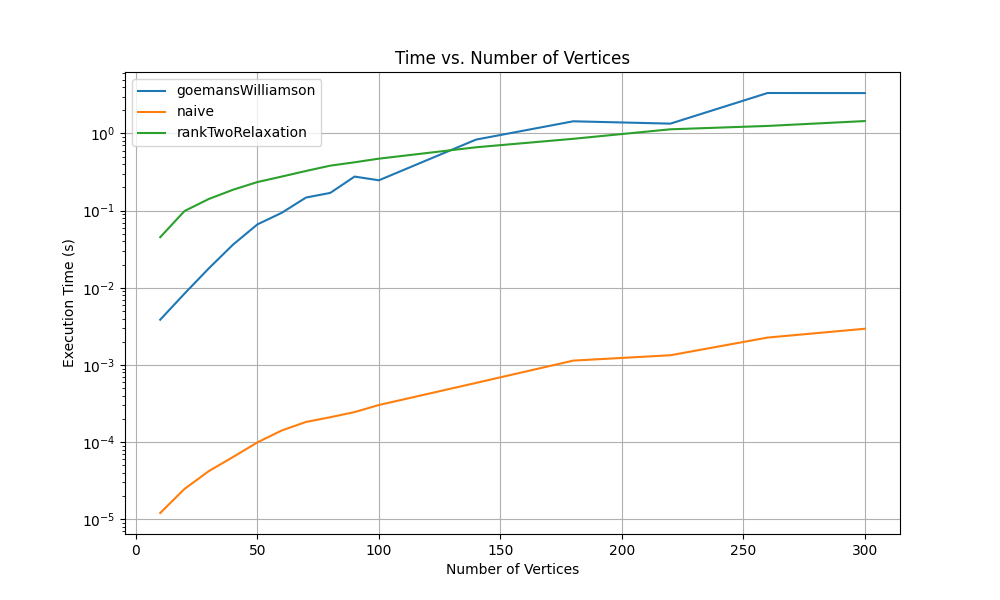
\includegraphics[width=\textwidth]{chapters/benchmark/Sections/images/cut/num_of_v/time_vs_vertices.png}
\caption{ Randomized graphs with edges chosen uniformly. }
\end{figure}

\begin{figure}[H]
\centering
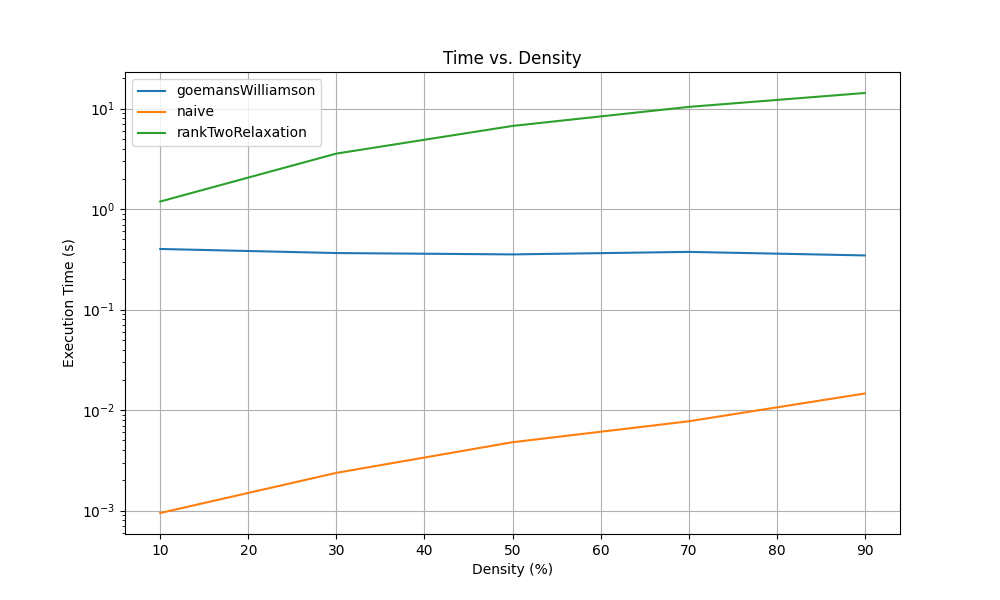
\includegraphics[width=\textwidth]{chapters/benchmark/Sections/images/cut/density/time_vs_density.png}
\caption{ Randomized graphs with edges chosen uniformly (\(|V| = 100\)).}
\end{figure}

\begin{figure}[H]
\centering
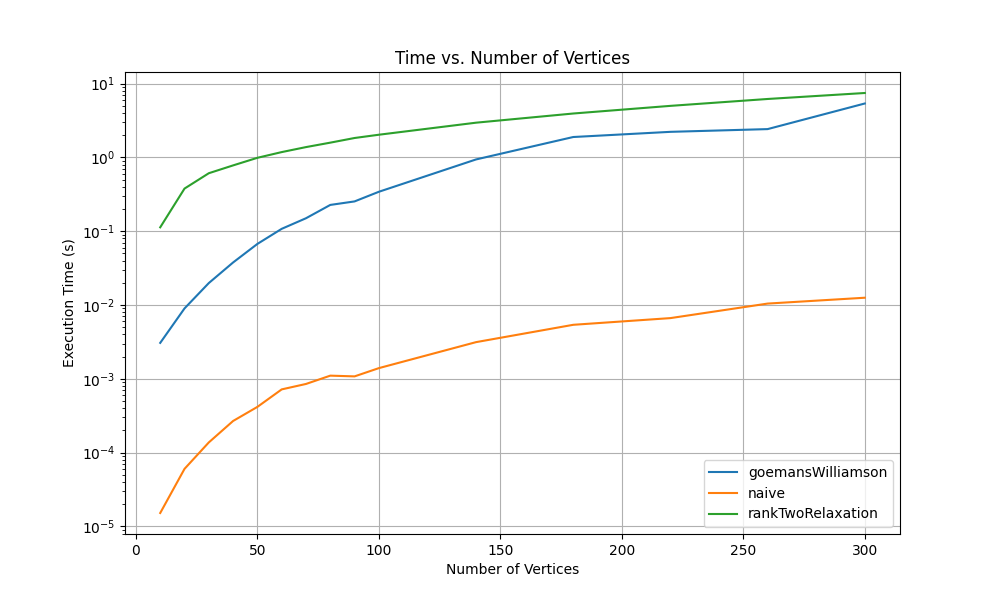
\includegraphics[width=\textwidth]{chapters/benchmark/Sections/images/cut/edges_times_8/time_vs_vertices.png}
\caption{ Randomized graphs with edges chosen uniformly (\(|E| = 8 \cdot |V|\)).}
\end{figure}

\begin{figure}[H]
\centering
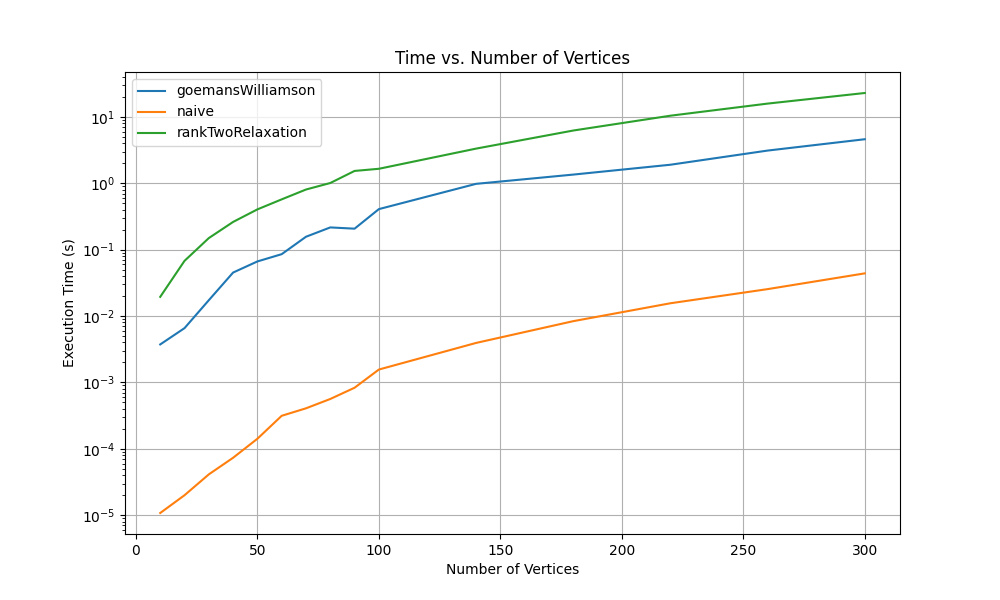
\includegraphics[width=\textwidth]{chapters/benchmark/Sections/images/cut/edges_square_dev_16/time_vs_vertices.png}
\caption{ Randomized graphs with edges chosen uniformly (\(|E| = \frac{|V|^2}{16}\)).}
\end{figure}

\begin{figure}[H]
\centering
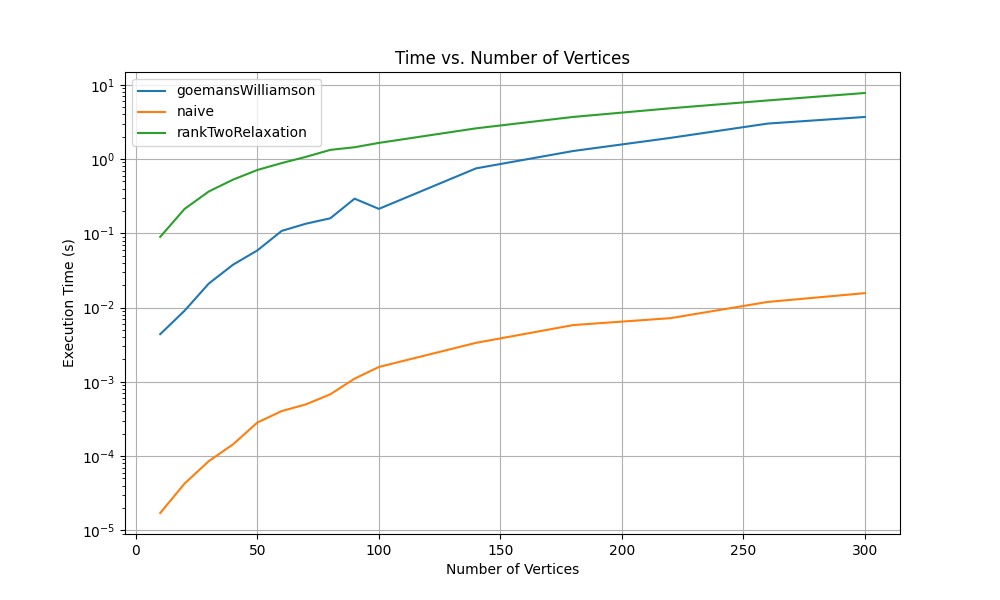
\includegraphics[width=\textwidth]{chapters/benchmark/Sections/images/cut/edges_v_times_log/time_vs_vertices.png}
\caption{ Randomized graphs with edges chosen uniformly (\(|E| = |V| \cdot \log{|V|}\)).}
\end{figure}

\begin{figure}[H]
\centering
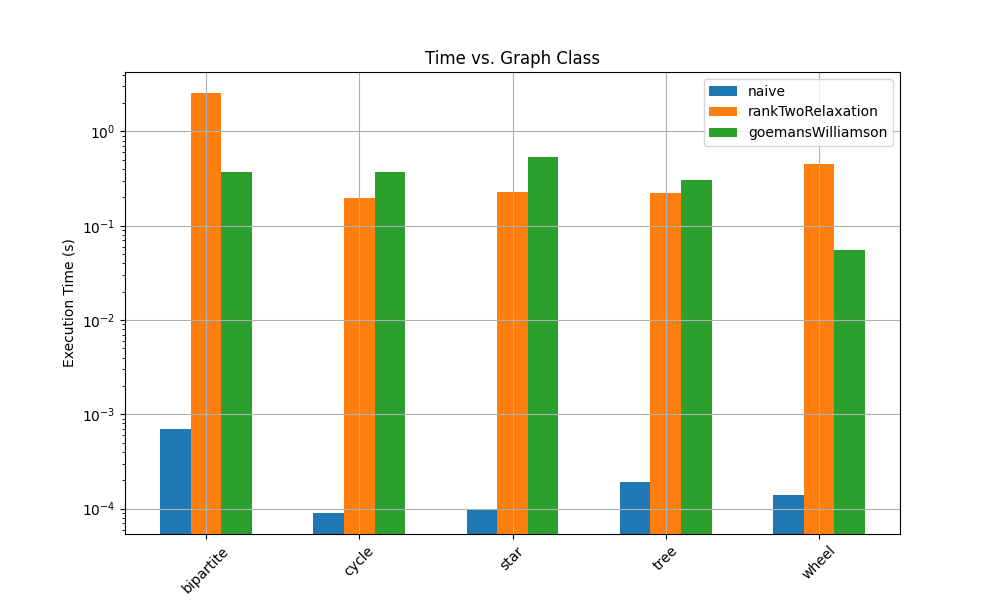
\includegraphics[width=\textwidth]{chapters/benchmark/Sections/images/cut/graph_types/time_vs_graph_class.png}
\caption{ Randomized graphs with edges chosen uniformly (\(|V| = 100\)).}
\end{figure}

\begin{figure}[H]
\centering
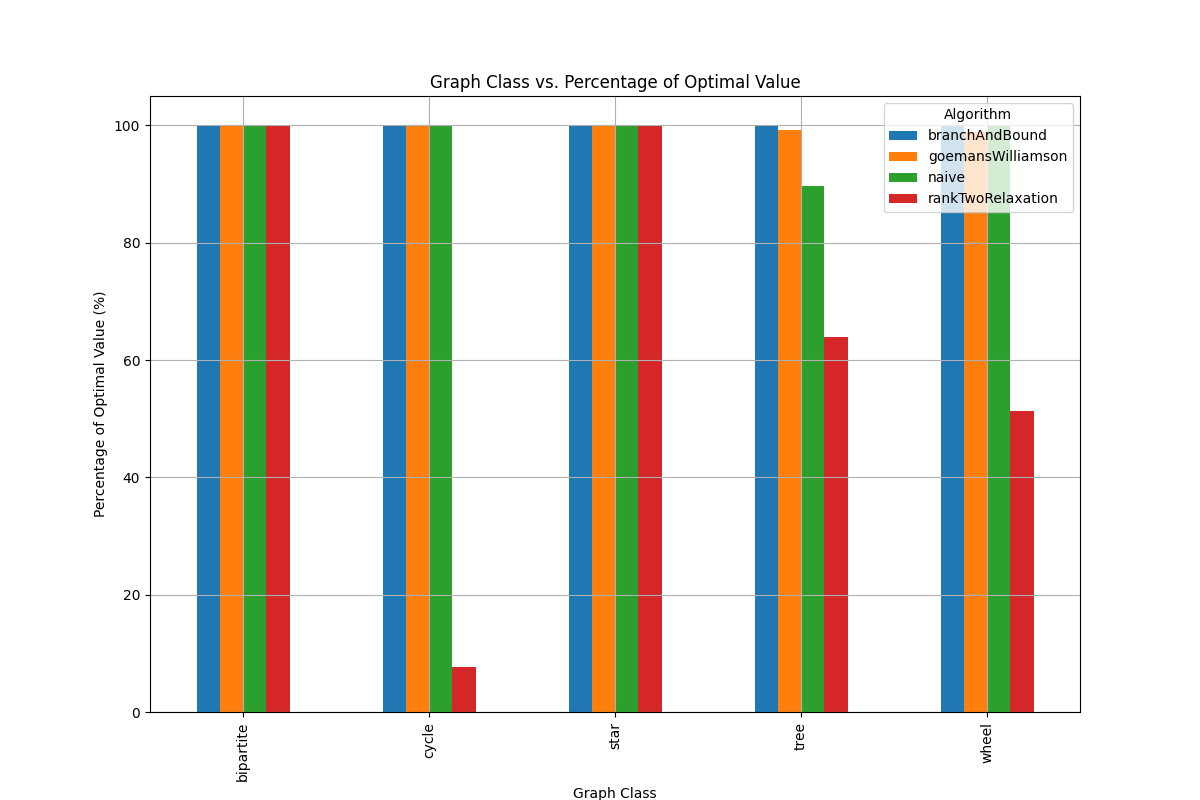
\includegraphics[width=\textwidth]{chapters/benchmark/Sections/images/cut/graph_types/graph_class_vs_percentage_optimal.png}
\caption{ Randomized graphs with edges chosen uniformly (\(|V| = 100\)).}
\end{figure}

\begin{figure}[H]
\centering
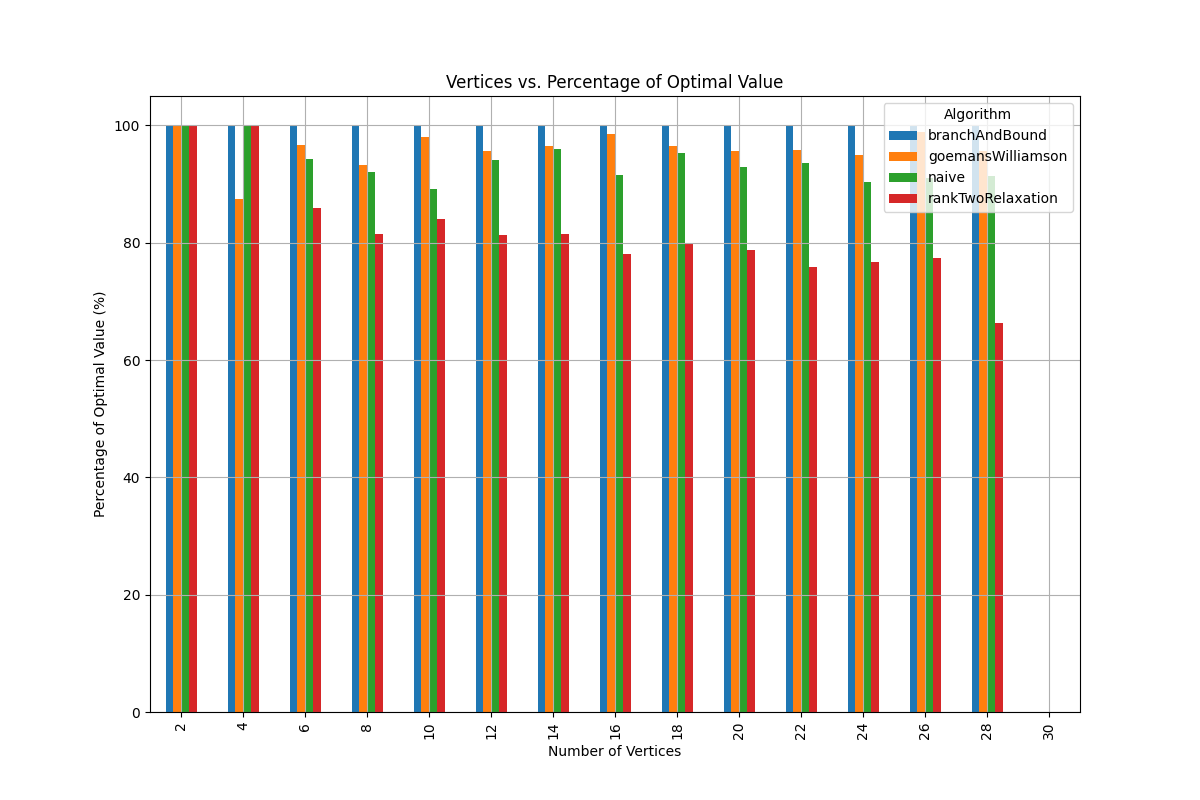
\includegraphics[width=\textwidth]{chapters/benchmark/Sections/images/cut/small_graphs/vertices_vs_percentage_optimal.png}
\caption{ Randomized graphs with edges chosen uniformly.}
\end{figure}


% Instances

\begin{table}[h!]
\centering
\caption{Max-cut instances benchmark results (time in seconds)}
\begin{tabular}{@{}lccccccc@{}}
\toprule
\textbf{Instance} & \multicolumn{2}{c}{\textbf{Greedy}} & \multicolumn{2}{c}{\textbf{Burer}} & \multicolumn{2}{c}{\textbf{Goemans-Williamson}} \\ 
\cmidrule(lr){2-3} \cmidrule(lr){4-5} \cmidrule(lr){6-7}
 & \textbf{Result} & \textbf{Time} & \textbf{Result} & \textbf{Time} & \textbf{Result} & \textbf{Time} \\ \midrule
be250 & \num{2.19e+05} & \num{1.66e-02} & \num{1.71e+05} & \num{1.18e+01} & \num{2.14e+05} & \num{4.67e-01} \\ 
bqp250 & \num{4.15e+05} & \num{2.05e-02} & \num{3.91e+04} & \num{1.12e+01} & \num{4.06e+05} & \num{6.02e-01} \\ 
deconv3x3 & \num{1.42e+07} & \num{2.66e-01} & \num{1.16e+05} & \num{1.42e+02} & \num{1.89e+07} & \num{1.99e+02} \\ 
hassan & \num{5.41e+06} & \num{1.89e-04} & \num{9.30e+05} & \num{7.56e-01} & \num{5.02e+06} & \num{3.46e-02} \\ 
house & \num{2.32e+05} & \num{3.27e-05} & \num{3.43e+04} & \num{2.51e-01} & \num{1.96e+05} & \num{1.22e-02} \\ 
HR\_G1 & \num{8.93e+05} & \num{6.55e-01} & \num{2.16e+05} & \num{1.16e+02} & \num{8.88e+05} & \num{1.67e+01} \\ 
matching & \num{2.61e+06} & \num{1.91e-04} & \num{7.33e+05} & \num{1.18e-2} & \num{2.78e+06} & \num{6.44e-03} \\ 
motor & \num{2.91e+05} & \num{1.88e-04} & \num{1.62e+04} & \num{9.92e-01} & \num{2.67e+05} & \num{6.99e-02} \\ 
sg3dl & \num{4.72e+04} & \num{8.07e-02} & \num{3.18e+03} & \num{9.72e+00} & \num{4.79e+04} & \num{6.13e+01} \\ 
superRes & \num{1.82e+09} & \num{1.02e+01} & \num{1.08e+08} & \num{1.88e+02} & \num{1.91e+09} & \num{3.11e+02} \\ 
\bottomrule
\end{tabular}
\end{table}

\subsubsection{Summary}

From the benchmarks performed, we observe that among the approximate algorithms, Goemans-Williamson and the naive algorithms gives the best results. However, as the number of vertices increases, the performance gap between these two algorithms rises. The runtime of the Goemans-Williamson and Burer algorithms are comparable to each other and become extremely slow for graphs with more than 10000 vertices. Consequently, for very large graphs, it is more efficient to use Karger's algorithm. On the other hand, for smaller graphs, the Goemans-Williamson algorithm is a prior choice. The time complexities and outcomes are consistent with our expectations based on the analysis.



\subsection{Min-cut}

% \begin{figure}[H]
% \centering
% 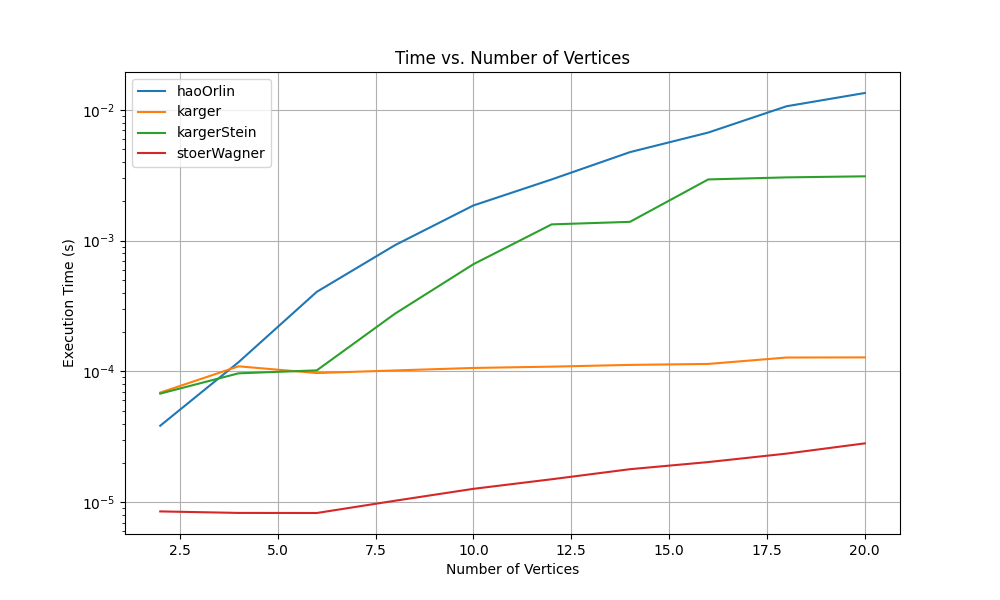
\includegraphics[width=\textwidth]{chapters/benchmark/Sections/images/min-cut/small_graphs/time_vs_vertices.png}
% \end{figure}

\begin{figure}[H]
\centering
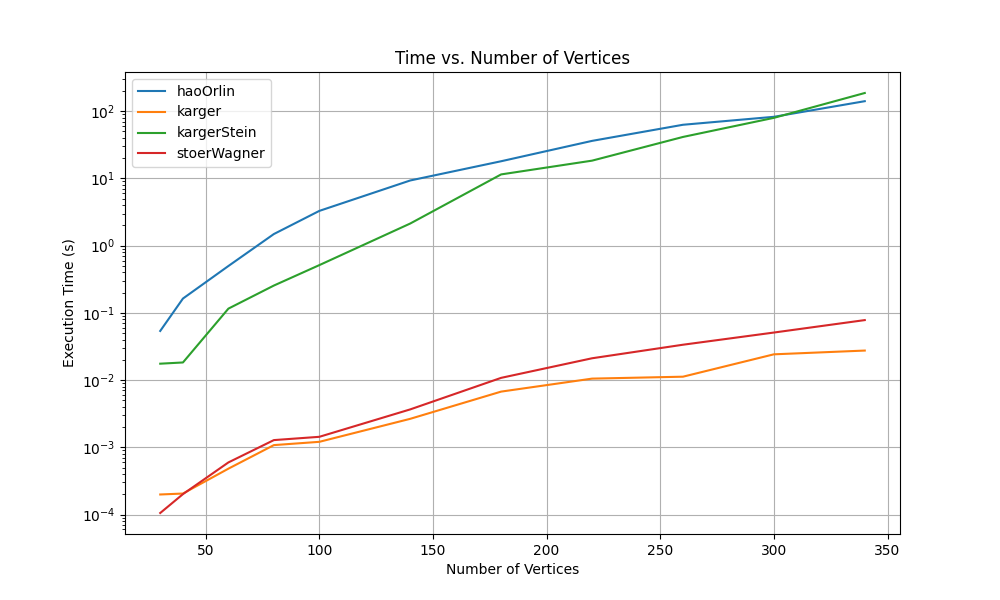
\includegraphics[width=\textwidth]{chapters/benchmark/Sections/images/min-cut/num_of_v/time_vs_vertices.png}
\caption{ Randomized graphs with edges chosen uniformly. }
\end{figure}

\begin{figure}[H]
\centering
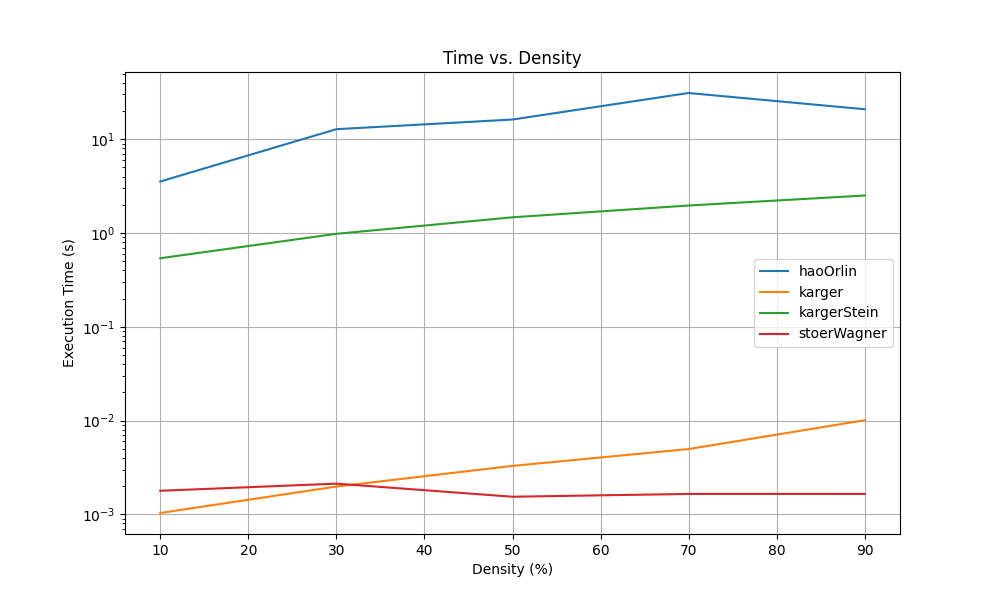
\includegraphics[width=\textwidth]{chapters/benchmark/Sections/images/min-cut/density/time_vs_density.png}
\caption{ Randomized graphs with edges chosen uniformly (\(|V| = 100\)).}
\end{figure}

\begin{figure}[H]
\centering
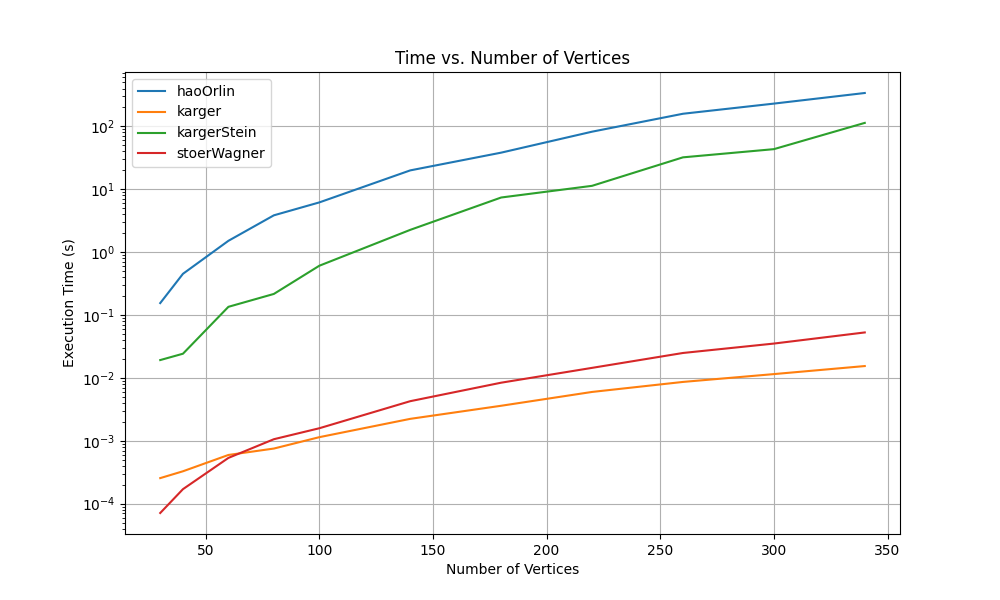
\includegraphics[width=\textwidth]{chapters/benchmark/Sections/images/min-cut/edges_times_8/time_vs_vertices.png}
\caption{ Randomized graphs with edges chosen uniformly (\(|E| = 8 \cdot |V|\)).}
\end{figure}

\begin{figure}[H]
\centering
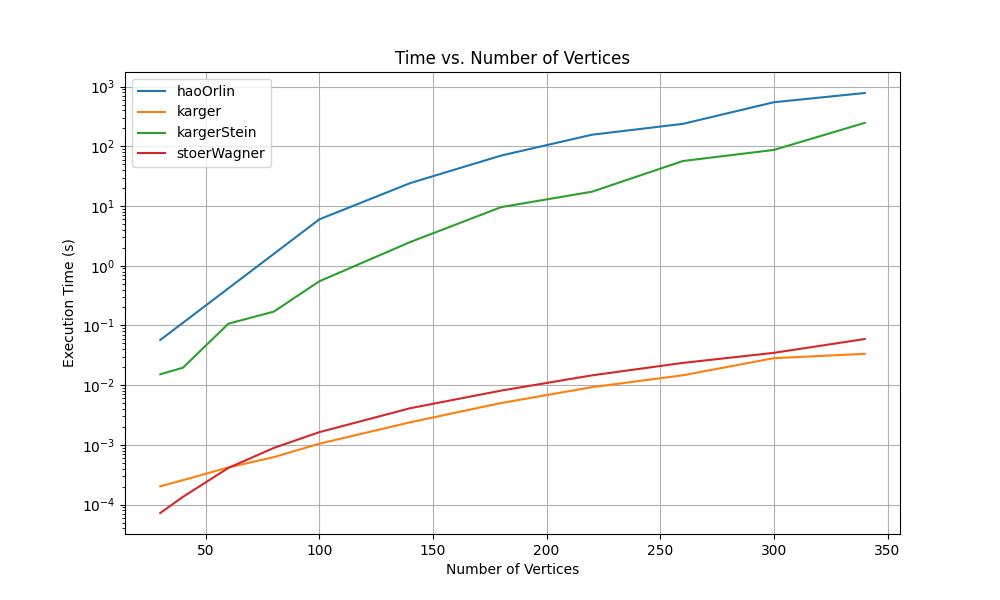
\includegraphics[width=\textwidth]{chapters/benchmark/Sections/images/min-cut/edges_square_dev_16/time_vs_vertices.png}
\caption{ Randomized graphs with edges chosen uniformly (\(|E| = \frac{|V|^2}{16}\)).}
\end{figure}

\begin{figure}[H]
\centering
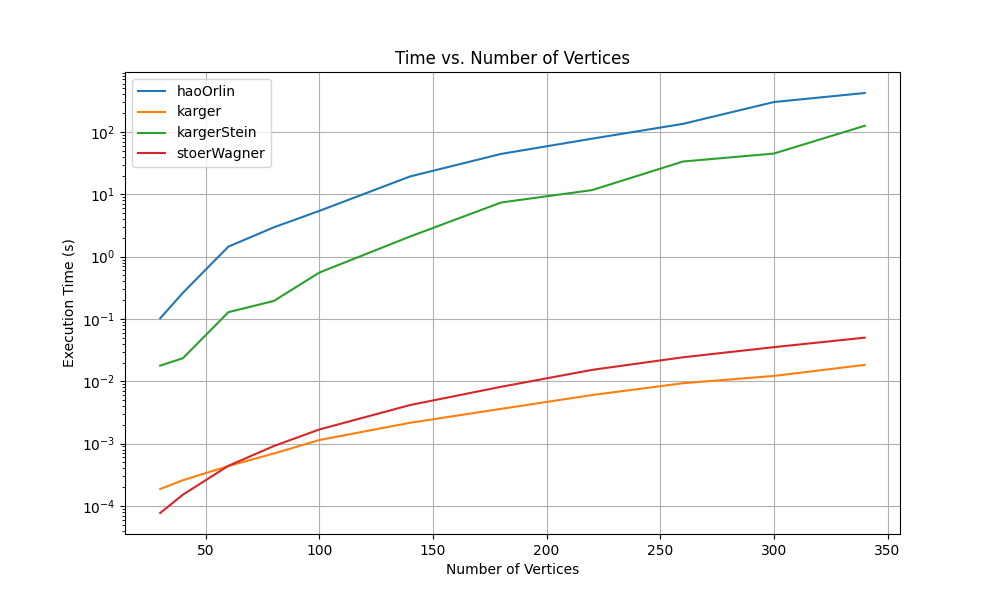
\includegraphics[width=\textwidth]{chapters/benchmark/Sections/images/min-cut/edges_v_times_log/time_vs_vertices.png}
\caption{ Randomized graphs with edges chosen uniformly (\(|E| = |V| \cdot \log{|V|}\)).}
\end{figure}

\begin{figure}[H]
\centering
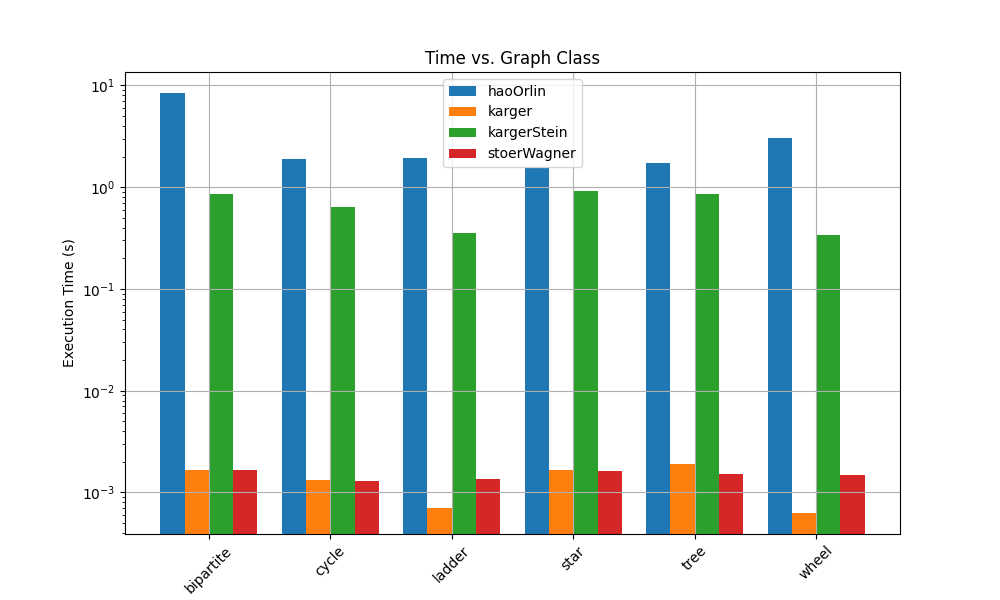
\includegraphics[width=\textwidth]{chapters/benchmark/Sections/images/min-cut/graph_types/time_vs_graph_class.png}
\caption{ Randomized graphs with edges chosen uniformly (\(|V| = 100\)).}
\end{figure}

% \begin{figure}[H]
% \centering
% 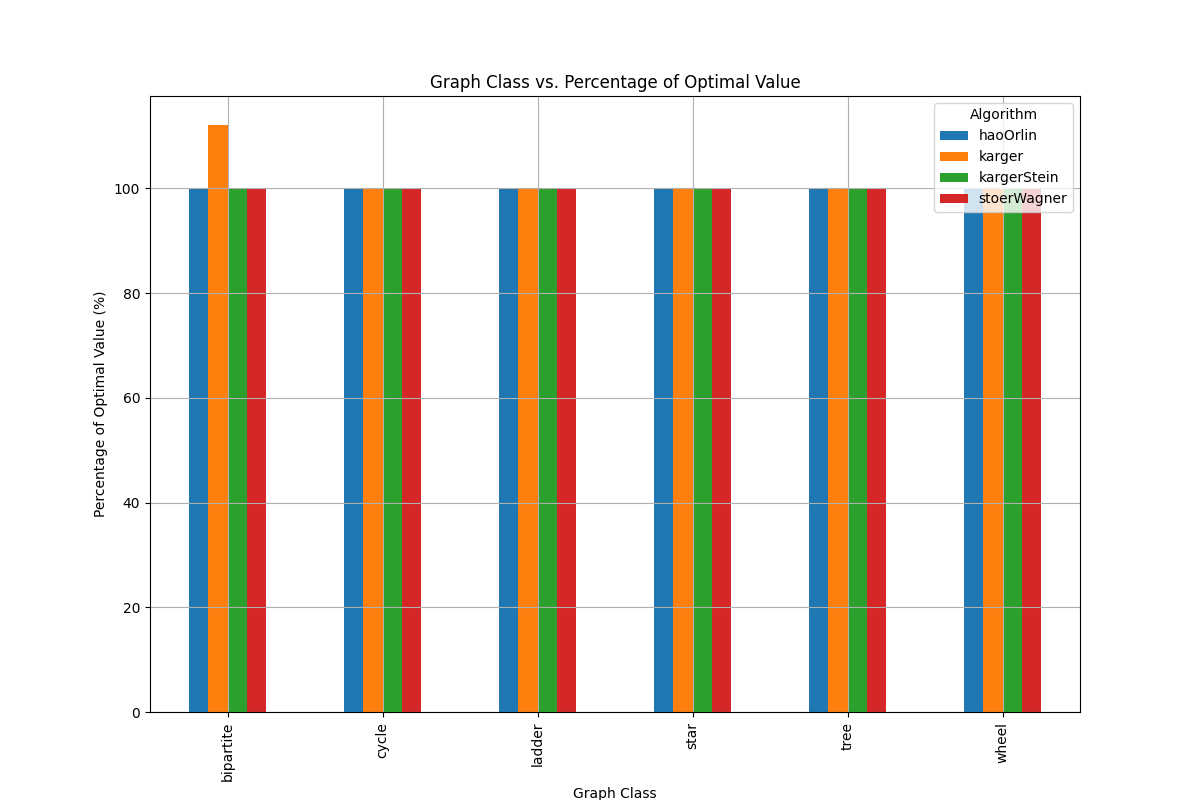
\includegraphics[width=\textwidth]{chapters/benchmark/Sections/images/min-cut/graph_types/graph_class_vs_percentage_optimal.png}
% \end{figure}

% \begin{figure}[H]
% \centering
% 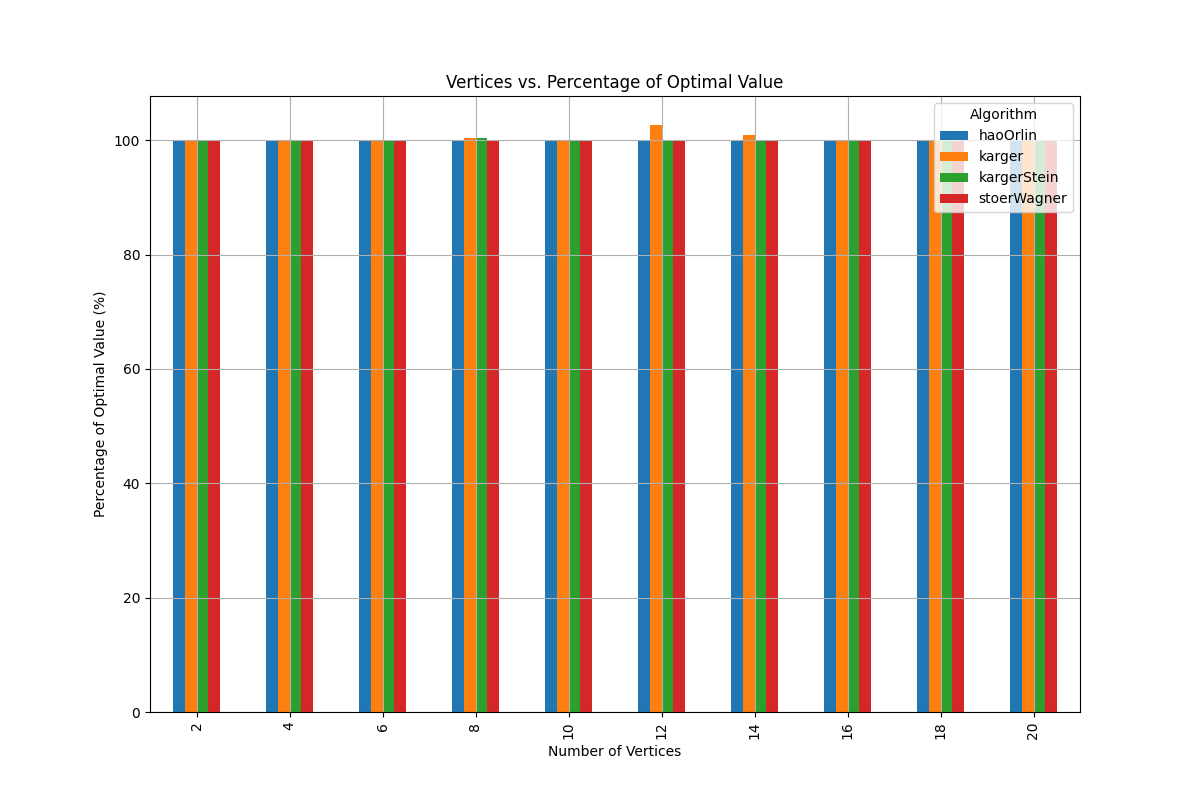
\includegraphics[width=\textwidth]{chapters/benchmark/Sections/images/min-cut/small_graphs/vertices_vs_percentage_optimal.png}
% \end{figure}



% Instances

\begin{table}[h!]
\centering
\caption{Min-cut instances benchmark results (time in seconds)}
\begin{tabular}{@{}lcccc@{}}
\toprule
\textbf{Instance} & \multicolumn{2}{c}{\textbf{Hao-Orlin}} & \multicolumn{2}{c}{\textbf{Karger}} \\ 
\cmidrule(lr){2-3} \cmidrule(lr){4-5}
 & \textbf{Result} & \textbf{Time} & \textbf{Result} & \textbf{Time} \\ \midrule
be250 & \num{1.42e+03} & \num{2.19e+02} & \num{1.42e+03} & \num{1.29e-02} \\ 
bqp250 & \num{2.41e+03} & \num{2.83e+02} & \num{2.41e+03} & \num{1.00e-02} \\ 
matching & \num{6.02e+04} & \num{2.42e-01} & \num{6.02e+04} & \num{2.72e-04} \\ 
motor & \num{3.00e+01} & \num{2.33e+00} & \num{3.00e+01} & \num{1.23e-02} \\ 
deconv\_graph3x3 & \num{5.38e+03} & \num{7.24e+03} & \num{5.86e+03} & \num{1.13e+01} \\ 
HR\_G1 & \num{2.13e+03} & \num{8.13e+03} & \num{2.69e+03} & \num{2.07e-01} \\ 
sg3dl & \num{8.40e+01} & \num{7.61e+03} & \num{8.40e+01} & \num{5.79e-02} \\ 
\bottomrule
\end{tabular}
\end{table}

\begin{table}[h!]
\centering
\begin{tabular}{@{}lcccc@{}}
\toprule
\textbf{Instance} & \multicolumn{2}{c}{\textbf{Karger-Stein}} & \multicolumn{2}{c}{\textbf{Stoer-Wagner}} \\ 
\cmidrule(lr){2-3} \cmidrule(lr){4-5}
 & \textbf{Result} & \textbf{Time} & \textbf{Result} & \textbf{Time} \\ \midrule
be250 & \num{1.42e+03} & \num{4.55e+01} & \num{1.42e+03} & \num{1.83e-02} \\ 
bqp250 & \num{2.41e+03} & \num{3.96e+01} & \num{2.41e+03} & \num{1.88e-02} \\ 
matching & \num{6.02e+04} & \num{2.28e-02} & \num{6.02e+04} & \num{1.30e-04} \\ 
motor & \num{3.00e+01} & \num{3.13e+00} & \num{3.00e+01} & \num{7.37e-04} \\ 
deconv\_graph3x3 & \num{5.57e+03} & \num{5.23e+03} & \num{5.38e+03} & \num{1.05e+01} \\ 
HR\_G1 & \num{2.13e+03} & \num{7.16e+03} & \num{2.13e+03} & \num{6.22e-01} \\ 
sg3dl & \num{8.40e+01} & \num{4.15e+03} & \num{8.40e+01} & \num{1.23e+00} \\ 
\bottomrule
\end{tabular}
\end{table}

\subsubsection{Summary}

From the benchmarks conducted on the min-cut algorithms, we observe that the Stoer-Wagner and Karger algorithms are the fastest. All algorithms produced approximately correct results, showcasing that the numerous iterations performed by Karger and Karger-Stein algorithms indicated correct results. The time complexities and outcomes are consistent with our expectations based on the analysis.
